% Геометрические примитивы.
\subsection{Геометрические примитивы, используемые в главе}

\subsubsection{Основные понятия}

При рассмотрении геометрических объектов наряду с понятием точки $P = (P_x, P_y, P_z) = (x_P, y_P, z_P)$ будем использовать также понятие радиус-вектора $\overline{P}$, компонентами которого являются координаты этой точки.
В дальнейшем будем считать эти термины взаимозаменяемыми.

Прямую, проходящую через точку $A$ (радиус-вектор $\overline{A}$) и направленную вдоль вектора $\overline{D}$, обозначаемую $Line(\overline{A}, \overline{D})$, будем определять как геометрическое место точек\label{term:gmt} (ГМТ\label{abbr:gmt}) $\overline{P}(\alpha)$ в пространстве, заданное следующим образом:
\begin{equation}\label{eqn:text_1_geo_prim_line}
	\overline{P}(\alpha) = \overline{A} + \alpha \overline{D}, \ \alpha \in \mathbb{R}.
\end{equation}

Отрезок с концами $A$, $B$ (с радиус-векторами $\overline{A}$, $\overline{B}$ соотвественно), обозначаемый $Segm(\overline{A}, \overline{B})$, будем определять как ГМТ $\overline{P}(\alpha)$ в пространстве, заданное следующим образом:
\begin{equation}\label{eqn:text_1_geo_prim_segment}
	\left\{
		\begin{aligned}
			& \overline{P}(\alpha) = \overline{A} + \alpha (\overline{B} - \overline{A}) = \overline{A} + \alpha \overline{AB} \\
			& 0 \le \alpha \le 1
		\end{aligned}
	\right.
\end{equation}

Треугольник с вершинами $A$, $B$, $C$ (с радиус-векторами $\overline{A}$, $\overline{B}$, $\overline{C}$ соответственно), обозначаемый $Tri(\overline{A}, \overline{B}, \overline{C})$, будем определять как ГМТ $\overline{P}(\beta, \gamma)$ в пространстве, заданное следующим образом:
\begin{equation}\label{eqn:text_1_geo_prim_triangle}
	\left\{
		\begin{aligned}
			& \overline{P}(\beta, \gamma) = \overline{A} + \beta (\overline{B} - \overline{A}) + \gamma (\overline{C} - \overline{A}) = \overline{A} + \beta \overline{AB} + \gamma \overline{AC} \\
			& \beta \ge 0 \\
			& \gamma \ge 0 \\
			& \beta + \gamma \le 1
		\end{aligned}
	\right.
\end{equation}

Прямоугольный параллелепипед будем определять как ГМТ $\overline{P} = (x, y, z)$ в пространстве, удовлетворяющих следующей системе неравенств:
\begin{equation}\label{eqn:text_1_geo_prim_parallelepiped}
	\left\{
		\begin{aligned}
			& x_l \le x \le x_h \\
			& y_l \le y \le y_h \\
			& z_l \le z \le z_h
		\end{aligned}
	\right.
\end{equation}

Для такого прямоугольного параллелепипеда будем использовать обозначаение $Box([x_l, x_h], [y_l, y_h], [z_l, z_h])$.

Шар с центром в точке $\overline{C}$ и радиуса $R$, обозначаемый как $Ball(\overline{C}, R)$, будем определять как ГМТ $\overline{P}$, удовлетворяющих условию
\begin{equation}
	|\overline{P} - \overline{C}| \le R
\end{equation}

Сферу с центром в точке $\overline{C}$ и радиуса $R$, представляющую собой поверхность шара $Ball(\overline{C}, R)$ будем обозначать $Sphere(\overline{C}, R)$.

\begin{definition}
Пусть дано некоторое ГМТ $G$, на точках $\overline{P} \in G$ которого определена неотрицательная функция $R: G \rightarrow \mathbb{R}_{\ge 0}$.
Тогда \textbf{окрестностью}\label{term:envelope} $G$, заданной указанной функцией $R(\overline{P})$, будем называть ГМТ, определяемое следующим образом:
\begin{equation}
	O_R(G) = \{ \overline{P}: \exists \overline{C} \in G \implies \overline{P} \in Ball(\overline{C}, R(\overline{C})) \}
\end{equation}
\end{definition}

\subsubsection{Задача о пересечении треугольника и прямоугольного параллелепипеда в пространстве}\label{sec:text_1_geo_prim_tri_and_parallelepiped_int}

Пусть в пространстве определены треугольник $Tri(\overline{A}, \overline{B}, \overline{C})$ и прямоугольный параллелепипед $Box([x_l, x_h], [y_l, y_h], [z_l, z_h])$.
Требуется определить, имеют ли они общие точки.

\begin{figure}[ht]
	\centering
	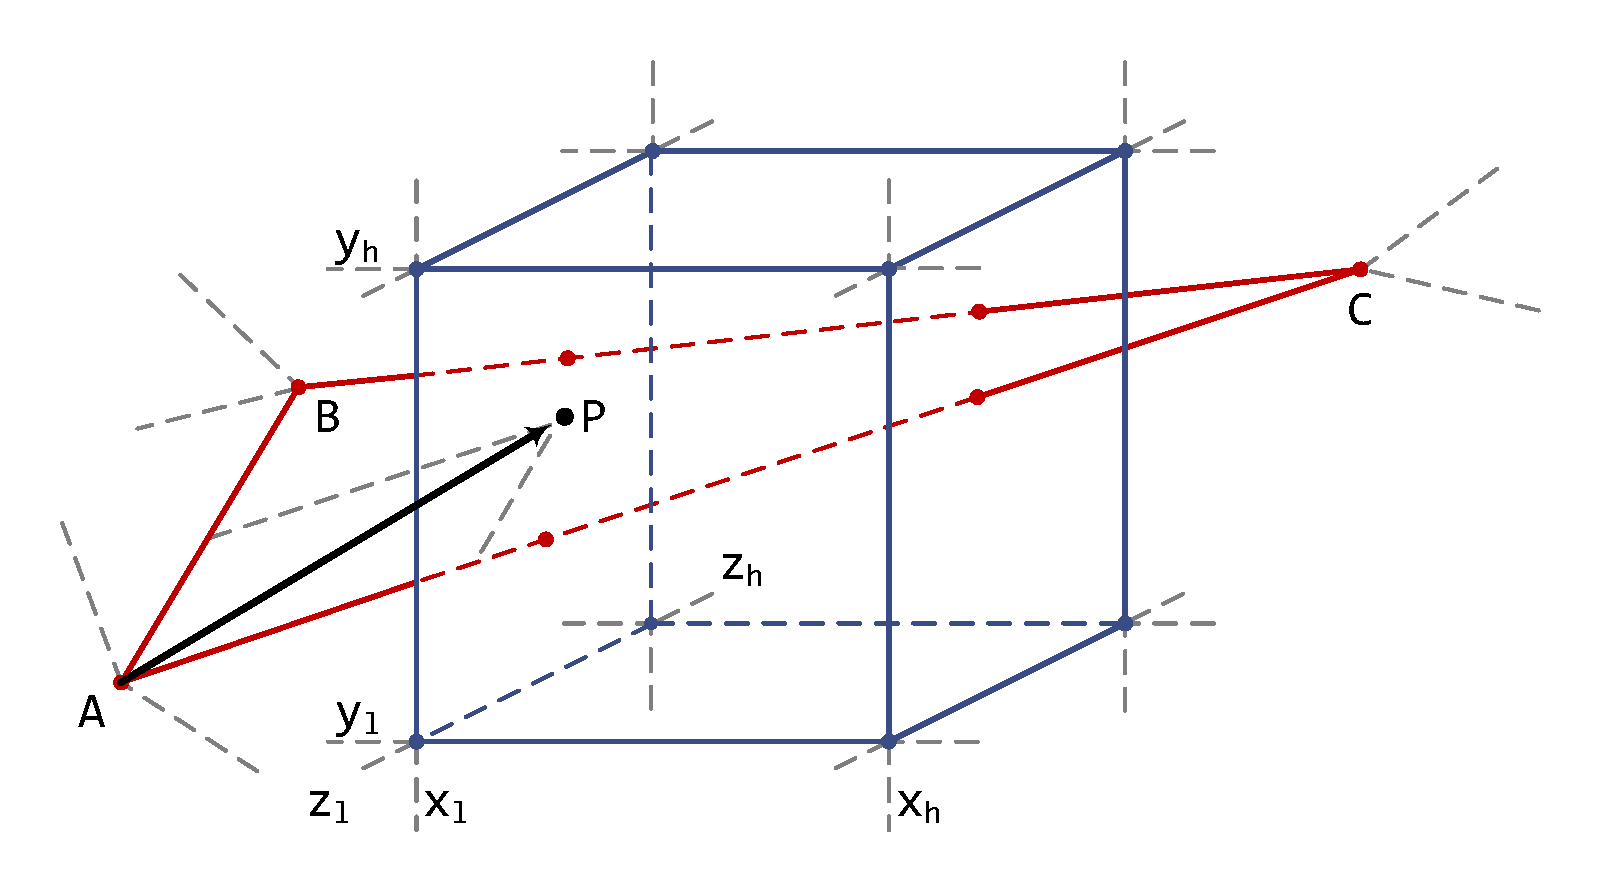
\includegraphics[width=0.7\textwidth]{./pics/text_1_geo_prim/tri_block_intersect.pdf}
	\caption{Пересечение прямоугольного параллелепипеда и треугольника.}
	\label{fig:text_1_geo_prim_tri_block_intersect}
\end{figure}

Для решения этой задачи подставим $\overline{P}(\beta, \gamma)$ из \eqref{eqn:text_1_geo_prim_triangle} в систему неравенств \eqref{eqn:text_1_geo_prim_parallelepiped}, получив следующую систему неравенств с двумя переменными $\beta$ и $\gamma$:
\begin{equation}\label{eqn:text_1_geo_prim_1}
	\left\{
		\begin{aligned}
			& x_l \le x_A + \beta (x_B - x_A) + \gamma (x_C - x_A) \le x_h \\
			& y_l \le y_A + \beta (y_B - y_A) + \gamma (y_C - y_A) \le y_h \\
			& z_l \le z_A + \beta (z_B - z_A) + \gamma (z_C - z_A) \le z_h \\
			& \beta \ge 0 \\
			& \gamma \ge 0 \\
			& \beta + \gamma \le 1
		\end{aligned}
	\right.
\end{equation}

Cистема \eqref{eqn:text_1_geo_prim_1} может быть решена методом свертывания конечных систем линейных неравенств \cite{Chernikov1963}.
Для применения метода свертывания систем линейных неравенств неравенства системы \eqref{eqn:text_1_geo_prim_1} необходимо привести к виду $k_{\beta}\beta + k_{\gamma}\gamma + k \le 0$, после чего получим следующую систему неравенств:
\begin{equation}\label{eqn:text_1_geo_prim_2}
	\left\{
		\begin{aligned}
			& (x_B - x_A) \beta + (x_C - x_A) \gamma + (x_A - x_h) \le 0 \\
			& (x_A - x_B) \beta + (x_A - x_C) \gamma + (x_l - x_A) \le 0 \\
			& (y_B - y_A) \beta + (y_C - y_A) \gamma + (y_A - y_h) \le 0 \\
			& (y_A - y_B) \beta + (y_A - y_C) \gamma + (y_l - y_A) \le 0 \\
			& (z_B - z_A) \beta + (z_C - z_A) \gamma + (z_A - z_h) \le 0 \\
			& (z_A - z_B) \beta + (z_A - z_C) \gamma + (z_l - z_A) \le 0 \\
			& -1 \cdot \beta + 0 \cdot \gamma \le 0 \\
			& 0 \cdot \beta + (-1) \cdot \gamma \le 0 \\
			& \beta + \gamma + (-1) \le 0
		\end{aligned}
	\right.
\end{equation}

Cистема неравенств \eqref{eqn:text_1_geo_prim_2} является системой с двумя переменными ($\beta$ и $\gamma$), поэтому после выполнения одного шага свертывания (деформации) она превратится в систему неравенств с одной переменной.
Деформация системы для исключения из нее переменной $\beta$ выполняется следующим образом.
Составляется новая система неравенств, в которую войдут все неравенства системы \eqref{eqn:text_1_geo_prim_2} вида $k_{\gamma} \gamma + k \le 0$, а каждая пара неравенств
\begin{equation}
	\begin{aligned}
		k_{\beta}^1 \beta + k_{\gamma}^1 \gamma + k^1 \le 0 \\
		k_{\beta}^2 \beta + k_{\gamma}^2 \gamma + k^2 \le 0
	\end{aligned}
\end{equation}

в которой коэффициенты при $\beta$ удовлетворяют неравенствам $k_{\beta}^1 < 0$ и $k_{\beta}^2 > 0$, войдет в деформированную систему неравенств в виде
\begin{equation}
	(k_{\gamma}^1 k_{\beta}^2 - k_{\gamma}^2 k_{\beta}^1) \gamma + (k^1 k_{\beta}^2 - k^2 k_{\beta}^1) \le 0. 
\end{equation}

Так как система \eqref{eqn:text_1_geo_prim_2} содержит 9 неравенств, из которых хотя бы в одном коэффициент при $\beta$ нулевой, не более чем в четырех –- положительный, и не более чем в четырех -- отрицательный, то в результате выполнения деформации получим систему, состоящую не более чем из 17 неравенств.
Если деформированная система неравенств с одной переменной имеет решение, то исходные треугольник и прямоугольный параллелепипед имеют общие точки.

\subsubsection{Задача поиска точек пересечения двух треугольников в пространстве}

Сначала рассмотрим задачу пересечения треугольника и отрезка в пространстве.
Пусть в пространстве задан треугольник $Tri(\overline{A}, \overline{B}, \overline{C})$ и отрезок $Segm(\overline{P}, \overline{Q})$.
Для поиска точек пересечения этого треугольника и отрезка требуется найти решение следующей системы уравнений
\begin{equation}\label{eqn:text_1_geo_prim_tri_segm_int}
	\left\{
		\begin{aligned}
			& x_A + (x_B - x_A) \beta + (x_C - x_A) \gamma = x_P + (x_Q - x_P) \alpha \\
			& y_A + (y_B - y_A) \beta + (y_C - y_A) \gamma = y_P + (y_Q - y_P) \alpha \\
			& z_A + (z_B - z_A) \beta + (z_C - z_A) \gamma = z_P + (z_Q - z_P) \alpha
		\end{aligned}
	\right.
\end{equation}

при ограничениям $0 \le \alpha \le 1$, $\beta \ge 0$, $\gamma \ge 0$, $\beta + \gamma \le 1$.

Система уравнений \eqref{eqn:text_1_geo_prim_tri_segm_int} может не иметь решений, может иметь ровно одно решение (если прямая $Line(\overline{P}, \overline{PQ})$ пересекает плоскость треугольника) либо имеет бесконечное количество решений (если прямая $Line(\overline{P}, \overline{PQ})$ лежит в плоскости треугольника.

\begin{figure}[ht]
	\centering
	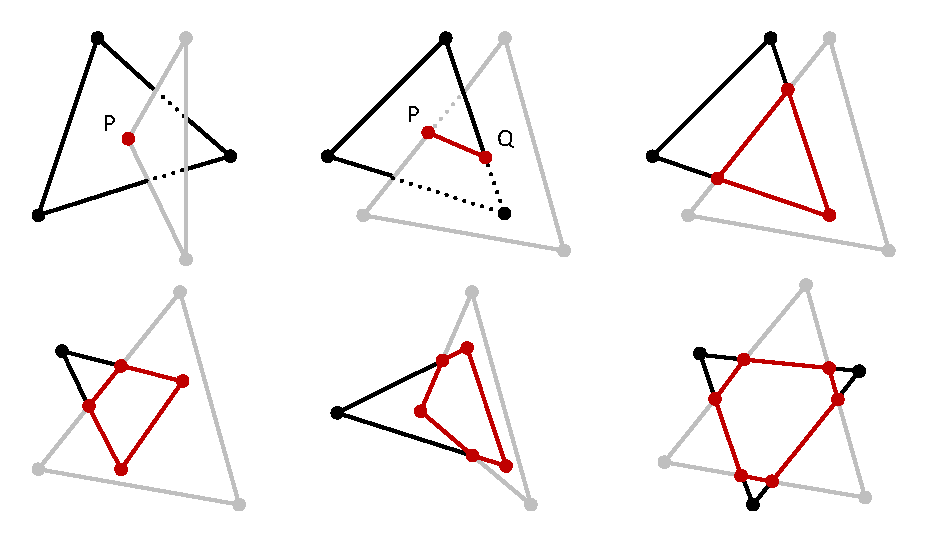
\includegraphics[width=0.7\textwidth]{./pics/text_1_geo_prim/tri_tri.pdf}
	\caption{Пересечение двух треугольников в пространстве.}
	\label{fig:text_1_geo_prim_tri_tri}
\end{figure}

Пусть теперь в пространстве заданы два треугольника.
Так как треугольник является выпуклой фигурой, то пересечение двух треугольников либо пусто, либо также является выпуклой фигурой (это может быть плоская фигура с количеством вершин от 1 до 6, см. рис.~\ref{fig:text_1_geo_prim_tri_tri}).

Вершины области пересечения двух треугольников это точки пересечения трех сторон первого треугольника со вторым треугольником и наоборот.
То есть для поиска вершин области пересечения двух треугольников нужно решить 6 задач пересечения треугольника с отрезком в пространстве.

\subsubsection{Задача поиска точек пересечения прямой с окрестностью отрезка}\label{sec:text_1_geo_prim_line_eps_intersect}

Пусть в пространстве задан отрезок $Segm(\overline{A}, \overline{B})$ согласно \eqref{eqn:text_1_geo_prim_segment}.
На точках этого отрезка $\overline{C}(\alpha) = \overline{A} + \alpha \overline{AB}, \ 0 \le \alpha \le 1$ задана функция $R(\overline{C}(\alpha))$ такая, что:
\begin{equation}
	\left\{
		\begin{aligned}
			& R(\overline{A}) = R_A \\
			& R(\overline{B}) = R_B \\
			& R(\overline{C}(\alpha)) = R(\alpha) = R_A + \alpha (R_B - R_A) = R_A + \alpha \Delta R
		\end{aligned}
	\right.
\end{equation}

Также пусть в пространстве задана прямая согласно \eqref{eqn:text_1_geo_prim_line}.
Без ограничения общности можно считать, что эта прямая проходит через начало координат, пусть она имеет вид $Line(\overline{0}, \overline{V}) = \{ \overline{P}(\tau) = \tau \overline{V}: \tau \in \mathbb{R} \}$.

Требуется найти точки пересечения прямой $Line(\overline{0}, \overline{V})$ и окрестности отрезка $O_R(Segm(\overline{A}, \overline{B}))$ \cite{Rybakov2017Flight}.

Точки пересечения прямой $Line(\overline{0}, \overline{V})$ и сферы с центром в точке $\overline{C}$ и радиусом $R$ находятся из решения системы уравнений
\begin{equation}\label{eqn:text_1_geo_prim_tv_pcr}
	\left\{
		\begin{aligned}
			& \overline{P} = \tau \overline{V} \\
			& |\overline{P} - \overline{C}| = R^2
		\end{aligned}
	\right.
\end{equation}

Система уравнений \eqref{eqn:text_1_geo_prim_tv_pcr} преобразуется в квадратное уравнение относительно $\tau$, дискриминант которого равен $4\left((\overline{C}, \overline{V})^2 - |\overline{V}|^2 \left(|\overline{C}|^2 - R^2\right)\right)$.
Общие точки прямой и сферы существуют если этот дискриминант неотрицателен.

Аналогично точки пересечения прямой $Line(\overline{0}, \overline{V})$ и сферы с центром в точке $\overline{C}(\alpha)$ и радиусом $R(\alpha)$ существуют, если выполняется условие
\begin{equation}
	(\overline{C}(\alpha), \overline{V})^2 - |\overline{V}|^2 \left(|\overline{C}(\alpha)|^2 - R(\alpha)^2\right) \ge 0.
\end{equation}

Подставив конкретные выражения для центра и радиуса сферы, получим квадратное неравенство относительно параметра $\alpha$:
\begin{equation}\label{eqn:text_1_geo_prim_ineq_k2k1k0}
	k_2 \alpha^2 + 2 k_1 \alpha + k_0 \ge 0,
\end{equation}

где
\begin{equation}\label{eqn:text_1_geo_prim_k2k1k0}
	\begin{aligned}
		& k_2 = (\Delta \overline{C}, \overline{V})^2 + |\overline{V}|^2 \left( \Delta R^2 - |\Delta \overline{C}|^2 \right) \\
		& k_1 = (\overline{C}_A, \overline{V})(\Delta \overline{C}, \overline{V}) + |\overline{V}|^2 \left(R_A \Delta R - (\overline{C}_A, \Delta \overline{C}) \right) \\
		& k_0 = (\overline{C}_A, \overline{V})^2 + |\overline{V}|^2 \left( R_A^2 - |\overline{C}_A|^2 \right)
	\end{aligned}
\end{equation}

В системе \eqref{eqn:text_1_geo_prim_k2k1k0} для удобства введены обозначения $\overline{C}_A = \overline{A}$, $\Delta \overline{C} = \overline{AB}$.

Неравентво \eqref{eqn:text_1_geo_prim_ineq_k2k1k0} может быть решено относительно $\alpha$, так как все коэффициенты из \eqref{eqn:text_1_geo_prim_k2k1k0} могут быть вычислены непосредственно.
Нас интересует решение неравенства \eqref{eqn:text_1_geo_prim_ineq_k2k1k0} только на отрезке $[0,1]$, оно представляет собой либо пустое множество, либо отрезок.
Если на отрезке $[0,1]$ неравенство \eqref{eqn:text_1_geo_prim_ineq_k2k1k0} не имеет решения, то прямая $Line(\overline{0}, \overline{V})$ не пересекает $O_R(Segm(\overline{A}, \overline{B}))$.
Допустим на отрезке $[0,1]$ неравенство \eqref{eqn:text_1_geo_prim_ineq_k2k1k0} имеет решение $[\alpha_0, \alpha_1] \subseteq [0, 1]$.
 
Для произвольного $\alpha \in [\alpha_0, \alpha_1]$ корни уравнения
\begin{equation}
	|\overline{V}|^2 \tau^2 - 2(\overline{C}(\alpha), \overline{V}) \tau + \left( |\overline{C}(\alpha)| - R(\alpha)^2 \right) = 0
\end{equation}

существуют и выражаются следующим образом:
\begin{equation}
	\tau_{1,2}(\alpha) = \frac{(\overline{C}(\alpha), \overline{V}) \pm \sqrt{k_2 \alpha^2 + 2 k_1 \alpha + k_0}}{|\overline{V}|^2}
\end{equation}

Искомые точки пересечения прямой $Line(\overline{0}, \overline{V})$ с границей окрестности отрезка $O_R(Segm(\overline{A}, \overline{B}))$ соответствуют минимальному и максимальному значениям параметра $\tau_{1,2}(\alpha)$, достигаемым на отрезке $[\alpha_0, \alpha_1]$.
Максимальное и минимальное значение $\tau_{1,2}(\alpha)$ могут достигаться либо на концах отрезка, либо в точках локального экстремума.
Для точки локального экстремума должно быть выполнено соотношение $\tau_{1,2}'(\alpha) = 0$ или в явном виде
\begin{equation}
	(\Delta \overline{C}, \overline{V}) \pm \frac{k_2 \alpha + k_1}{ \sqrt{k_2 \alpha^2 + 2 k_1 \alpha + k_0} } = 0
\end{equation}

Введя обозначение $q = (\Delta \overline{C}, \overline{V})$, получим квадратное уравнение относительно $\alpha$:
\begin{equation}
	k_2 (k_2 - q) \alpha^2 + 2 k_1 (k_2 - q) \alpha + (k_1^2 - q k_0) = 0,
\end{equation}

решая которое, получим потенциальные точки локальных экстремумов $\tilde{\alpha}_1$, $\tilde{\alpha}_2$.

Точки $\tilde{\alpha}_1$, $\tilde{\alpha}_2$ нужно учитывть только если они попадают в отрезок $[\alpha_0, \alpha_1]$.
В общем случае значения $\tau_{1,2}$ находятся по четырем значениям $\alpha$
\begin{equation}
	\left\{
		\begin{aligned}
			\tau_1 = \min(t_1(\alpha_0), t_1(\alpha_1), t_1(\tilde{\alpha}_0), t_1(\tilde{\alpha}_1)) \\
			\tau_2 = \max(t_2(\alpha_0), t_2(\alpha_1), t_2(\tilde{\alpha}_0), t_2(\tilde{\alpha}_1))
		\end{aligned}
	\right.
\end{equation}

Множеством общих точек $Line(\overline{0}, \overline{V})$ и $O_R(Segm(\overline{A}, \overline{B}))$ является $\{ \overline{P}(\tau): \tau_1 \le \tau \le \tau_2 \}$.

\begin{figure}[ht]
	\centering
	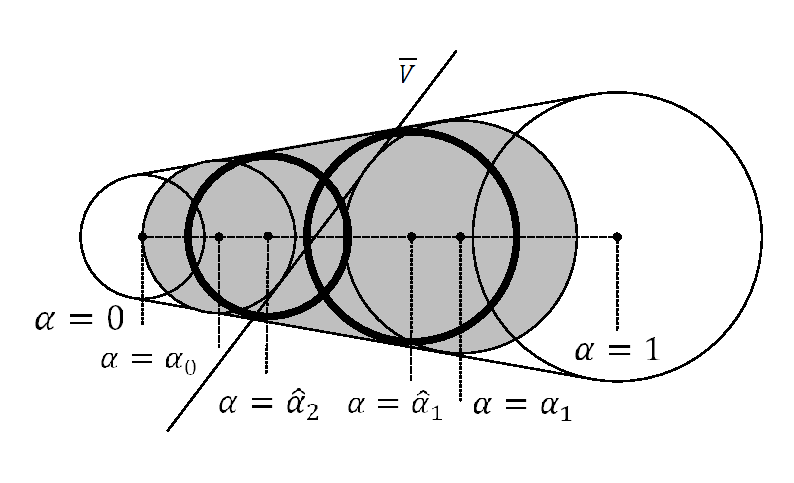
\includegraphics[width=0.80\textwidth]{./pics/text_1_geo_prim/spheres_nest_intersection.pdf}
	\caption{Пересечение прямой с окрестностью отрезка.}
	\label{fig:text_1_geo_prim_spheres_nest_intersection}
\end{figure}
